%\documentclass{article}
\documentclass[twocolumn]{article}
\usepackage[utf8]{inputenc}
\usepackage{tikz}
\usetikzlibrary{positioning,fit,shapes,arrows.meta}

\author{ K\'evin Le Bon \and Alan Schmitt }

\title{MLExplain}

\begin{document}
\maketitle

\begin{abstract}
  MLExplain is a step-by-step visual interpreter for OCaml that enables the
  user to inspect both their program's state and the interpreter's state
  itself. This interpreter aims to provide the user with a better understanding
  of the semantics of OCaml semantics.
\end{abstract}

\section{Introduction}

The semantics of a programming language can be very complex. When a language
has no specification, the semantics is then defined by the implementations of
the language, i.e., interpreters and compilers. However even when a
specification is available, it can be difficult to understand why the execution
of a specific program results to a certain output.

The project \emph{JSExplain} \cite{chargueraud:hal-01745792} aims
to describe a JavaScript program's execution by showing every step of an
interpreter which behavior is the closest to JavaScript specification. This
paper shows how we adapted JSExplain to OCaml.

Unlike JavaScript, OCaml has no official specification. However, OCaml code
execution is fairly simple because the amount of language constructions is
small. We have written an interpreter for OCaml's typed abstract syntax tree
(AST). This AST is close to source code and need little transformations but
supplies us with resolved names -- which is useful for module and signatures
inclusion and absolutely mandatory for features like named parameters in
functions.  The semantic we give to OCaml is higher level than the one
described in \emph{ZINC} \cite{Leroy-ZINC} virtual machine which is at the same
level as object code.

\section{The visual interpreter JSExplain}

An interpreter is a program that takes code written in a specific language as
input and execute it. In order to achieve its goal, the interpreter does
several analyses ; here are the most common : lexical analysis, parsing and
typing.

We call a \emph{visual interpreter} an interpreter that is able to display the
program's state, the current location in source and local-variable values at
each step of the execution as well as the state of the interpreter itself.
JSExplain is a visual interpreter for JavaScript. The aim of this tool is to
enable a user to better understand JavaScript's semantics. JSExplain's
interface highlights the expression of the program currently evaluated as well
as the instruction of the interpreter that is executed.

\section{JSExplain functioning}

JSExplain is a visual interpreter. To display its state, the interpreter is
compiled with a compiler that adds calls to a tracing function. The traced
retrieved during the execution of the program gives many information about the
state of the interpreter:

\begin{itemize}
  \item existing variables and their values
  \item return values of functions of the interpreter
\end{itemize}

JSExplain's web interface uses these traces in order to display the program and
interpreter state at every step of the execution.

The whole project takes the shape of a web application composed of the
JavaScript interpreter and a view. The view allows the user to write JavaScript
code and run it. It also displays the state of the program and the state of the
interpreter.

The program's execution is not interactive: when the button \texttt{run} is
pressed, the program is executed all at one and the traces are generated. Only
then, the user can replay the execution step by step.

\subsection{JSExplain's compiler}

% Référence pour coq ?
JSExplain was first written in Coq. OCaml code has been extracted from the Coq
source and is now the primary source code. The interpreter is compiled into
JavaScript in order to use it within a web page. For this reason, the project
embeds a homemade OCaml-to-JavaScript compiler.

JSExplain also needs its own OCaml to JavaScript compiler in order to place the
calls to \verb|log_event| which is the tracing function. This function is also
used to get the location of the different syntactical objects in the source
file in order to produce code highlighting in JSExplain's interface.

This compiler offers several compilation modes:

\begin{itemize}
  \item \texttt{unlog}: generate JavaScript without tracing.
  \item \texttt{log}: generate JavaScript with tracing.
  \item \texttt{mlloc}, \texttt{token} and \texttt{ptoken}: generate files with
    informations about syntastical elements from the input file.
  \item \texttt{pseudo}: generate JavaScript enhanced with syntactic sugar for
    pattern matching or monadic operations -- it is supposed to be easier to
    read.
\end{itemize}

Modes \texttt{unlog} and \texttt{log} exist so that auxiliary code in the
interpreter -- like linked-list or hash-map internal-management functions -- is
not traced.  The user is thus able to concentrate on the logical part of the
interpreter functioning and forget about implementation details.

\subsubsection{fOCaml}
This compiler does not recognized the whole OCaml language, it can only handle
a small subset we named \texttt{fOCaml}. Among other restrictions, it cannot
handle objects and imperative features, exceptions, inner modules, and tuples.
The main reason for this limitation is that compiling OCaml into JavaScript is
not trivial, many features -- e.g. nested pattern matching -- are hard to
represent to JavaScript.

The fOCaml code is compiled into \texttt{fJs}, a functional subset of
JavaScript. The compiler preserves as much as possible the code structure to
enable the user to understand both fOCaml and fJs codes as the same one.

% Petite explication sur le fait que du coup on écrit du code fonctionnel pur
% et les implications que ça a ?

\section{MLExplain}

At first glance, JSExplain seems tightly linked to JavaScript. However, the
architecture of the project actually allows us to take off the interpreter
completely and replace it with another one.

% Plus de blabla

\subsection{Two compilers}

To interpret OCaml code, we need to parse it. However, our compiler does not
allow us to use the standard library nor an external one.

\begin{figure*}[ht]
  \centering
  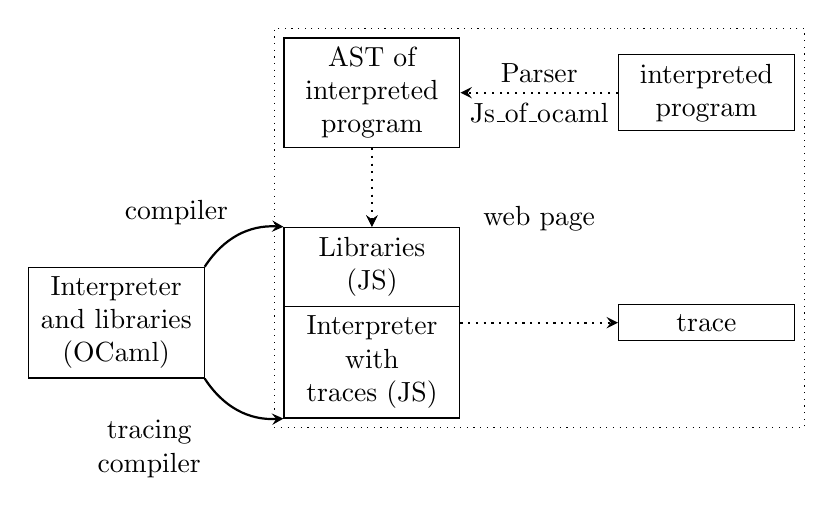
\begin{tikzpicture}[nodes = {align = center}]
    \node (focaml) [draw, text width=2cm] {Interpreter and libraries (OCaml)};

    \node (fjs) [draw, right = 1cm of focaml, text width=2cm, rectangle split,
    rectangle split parts=2, text centered] {Libraries (JS) \nodepart{second}
      Interpreter with traces (JS)};

    \node (ast) [draw, above = of fjs, text width=2cm] {AST of interpreted
      program};

    \node (source) [draw, right = 2cm of ast, text width=2cm, text centered]
    {interpreted program};

    \node [draw, dotted, fit=(fjs) (ast) (source)] {web page};

    \node (trace) [draw, right = 2cm of fjs, text width=2cm, text centered]
    {trace};

    \path[->,thick,>=stealth] (focaml.north
    east) edge[bend left] node[above left] {compiler} (fjs.north west) ;

    \path[->,thick,>=stealth] (focaml.south east) edge[bend right] node[below
    left] {\parbox{2cm}{\centering tracing compiler}} (fjs.south west);

    \path[->,thick,dotted,>=stealth] (source) edge node [above] {Parser} node
    [below] {Js\_of\_ocaml} (ast);

    \path[->,thick,dotted,>=stealth] (ast) edge (fjs);

    \path[->,thick,dotted,>=stealth] (ast) edge (fjs);

    \path[->,thick,dotted,>=stealth] (fjs) edge (trace);
  \end{tikzpicture}
  
  \caption{Architecture of MLExplain}
  \label{fig:archi}
\end{figure*}

\bibliographystyle{plain}
\bibliography{biblio}

\end{document}
